\section{Struktura dat a pojmy}

\subsection{Problémy}


\section{Požadavky}

Na základě předem popsaných problémů a hlavních požadavků jsem sestavil funkční a nefunkční požadavky pokrývající požadovanou funkcionalitu aplikace.

\subsection{Funkční}
% Co má systém umět

%\subsubsection{F1 -- Pomocník pro inicializaci obrazu softwaru Syllabus Plus}
%Pro inicializaci obrazu softwaru Syllabus Plus a další práci s daty je potřeba zadat informace o daném semestru.
%Správné nastavení je klíčové pro korektní plánování časových lístků.


\subsection{Nefunkční}

%\subsubsection{N1 -- Aplikace s grafickým uživatelským rozhraním}
%Aplikace by měla mít grafické uživatelské rozhraní pro práci s daty.
%Uživatel by tak měl být schopen obsluhovat aplikaci sám bez pomoci další osoby.

\section{Případy užití}


%\begin{figure}
%    \centering
%    \captionsetup{justification=centering}
%    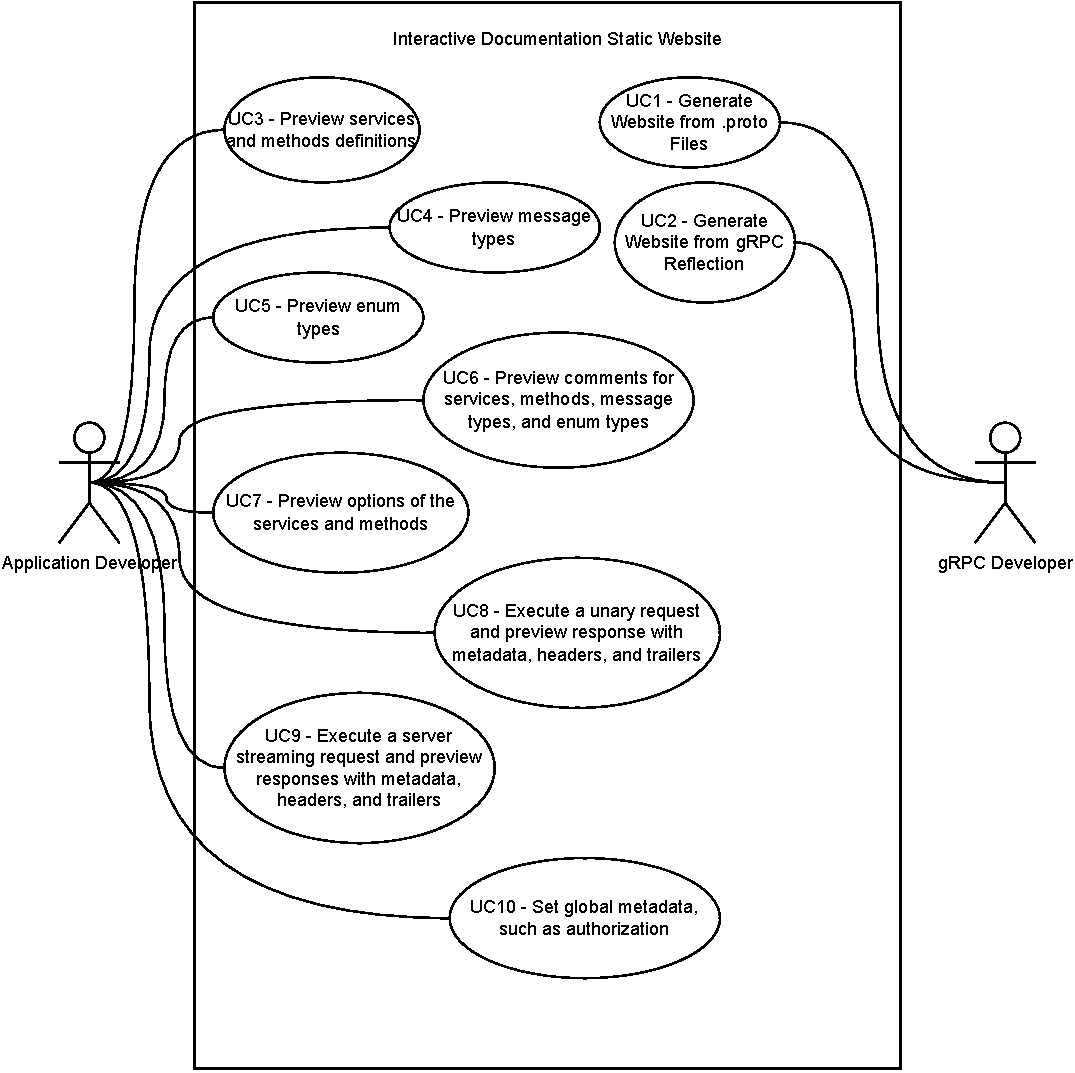
\includegraphics[width=1.0\textwidth]{use-case-diagram}
%    \caption{Diagram případů užití}
%    \label{fig:use-case-diagram}
%\end{figure}

%\subsection{UC1 -- Inicializace obrazu softwaru Syllabus Plus}
%Rozvrhář spustí software Syllabus Plus a začne s inicializací nového obrazu.
%Během inicializace se mu zobrazí dialog pro nastavení začátku semestru, vyučované dny, začátek a konec hodin, počet hodin za den a počet týdnů na semestr.
%Rozvrhář otevře aplikaci pro převod a nastaví semestr, který se využije pro načítání dat ze systému KOS\@.
%Zobrazí si jakým způsobem má položky nastavit, aby byla data správně reprezentována (například při plánování časových lístků).
%Formulář vyplní podle získaných dat z aplikace a inicializuje obraz.
%V případě, že se rozvrhář splete, musí aktuální obraz smazat a začít vytvářet nový od začátku.
%Jinak je inicializace úspěšně dokončena.


\section{Mapování požadavků na případy užití}
Sestavil jsem tabulku mapování požadavků a případu užití (viz tabulka~\ref{tab:use_cases}), abych si ověřil, že všechny požadavky jsou pokryty alespoň jedním případem užití a zároveň že žádný případ užití není zbytečný.
Tabulka ukazuje, že jsou všechny požadavky pokryty.

\begin{table}[hbt!]
    \centering
    \captionsetup{justification=centering}
    \begin{tabular}{|l|l|l|l|l|l|l|l|l|l|l|l|l|l|l|l|}
        \hline
        & \multicolumn{15}{c|}{Případy užití} \\ \hline
        & 1 & 2 & 3 & 4 & 5 & 6 & 7 & 8 & 9 & 10 & 11 & 12 & 13 & 14 & 15 \\ \hline
        F1  & x &   &   &   &   &   &   &   &   &    &    &    &    &    &    \\ \hline
        F2  &   &   & x &   &   &   &   &   &   &    &    &    &    &    &    \\ \hline
        F3  &   &   &   & x &   &   &   &   &   &    &    &    &    &    &    \\ \hline
        F4  &   &   &   &   &   &   &   &   &   &    &    &    &    &    & x  \\ \hline
        F5  &   &   &   &   & x &   &   &   &   &    &    &    &    &    &    \\ \hline
        F6  &   & x &   &   &   &   &   & x &   &    &    & x  & x  &    &    \\ \hline
        F7  &   & x &   &   &   &   &   &   &   &    &    & x  &    &    &    \\ \hline
        F8  &   &   &   &   &   &   &   &   &   &    &    &    & x  &    &    \\ \hline
        F9  &   & x &   &   &   &   &   &   &   &    & x  &    &    &    &    \\ \hline
        F10 &   & x &   &   &   &   &   &   &   &    &    &    &    &    &    \\ \hline
        F11 &   &   &   &   &   &   &   &   & x & x  &    &    &    &    &    \\ \hline
        F12 &   & x &   &   &   &   &   &   &   &    &    &    &    &    &    \\ \hline
        F13 &   &   &   &   &   &   &   &   &   & x  &    &    &    &    &    \\ \hline
        F14 &   &   &   &   &   &   &   & x & x & x  &    & x  & x  &    &    \\ \hline
        F15 &   &   &   &   &   &   &   & x & x & x  &    & x  &    &    &    \\ \hline
        F16 &   &   &   &   &   &   &   & x & x & x  &    & x  & x  &    &    \\ \hline
        F17 &   &   &   &   &   & x & x &   &   &    &    &    &    &    &    \\ \hline
        F18 &   &   &   &   &   & x &   &   &   & x  &    &    &    & x  &    \\ \hline
        F19 & x &   &   &   &   &   &   &   &   &    &    &    &    &    &    \\ \hline
    \end{tabular}
    \caption{Mapování požadavků a případů užití}
    \label{tab:use_cases}
\end{table}